\documentclass[11pt, a4paper]{article}

\usepackage[T2A]{fontenc}
\usepackage[utf8]{inputenc}
\usepackage[english, russian]{babel}
\usepackage{amssymb}
\usepackage{amsfonts}
\usepackage{amsmath}
\usepackage{mathtext}
\usepackage{comment}
\usepackage{graphicx}

\usepackage{tikz}
\usepackage{geometry}
\geometry{left=1cm, right=1cm, top=2cm, bottom=2cm}
\sloppy
\usepackage{wrapfig}
\graphicspath{{../../}}
\usepackage{fancybox,fancyhdr}

\newcommand{\head}[2]
{
	\fancyhf{}
	\pagestyle{fancy}
	\chead{Казахстанский филиал МГУ имени М.В.Ломоносова}

	\begin{center}
	\begin{LARGE}
	#1
	\end{LARGE}
	\end{center}

	\begin{center}
	\begin{large}
	#2
	\end{large}
	\end{center}

	\begin{center}
	\begin{LARGE}
	Указания
	\end{LARGE}
	\end{center}
}

\begin{document}

\head{Отборочная олимпиада по математике}{15 марта 2014}

\begin{enumerate}

\item Операцию деления пополам можно получить следующим образом: 
$$\frac{x}{2} = \frac{1}{\frac{1}{x} + \frac{1}{x}}$$
А операцию умножения так: 
$$a b = \left( \frac{a+b}{2} \right)^2 - \left( \frac{a-b}{2} \right)^2.$$

\item Ответ: 1. По теореме Виета: $\alpha \beta \gamma = 1$, $\alpha \beta + \beta \gamma + \gamma \alpha = -1$, $\alpha + \beta + \gamma = 0$.
Используя уравнения, заменим 
$$ \frac{1-\alpha}{1+\alpha} = \frac{\alpha^3 - 2 \alpha}{\alpha^3}.$$
Осталось заметить, что:
$$\frac{1}{\alpha^2} + \frac{1}{\beta^2} + \frac{1}{\gamma^2} = (\alpha \beta + \beta \gamma + \gamma \alpha)^2 - 2 (\alpha + \beta + \gamma) = 1.$$


\item Ответ: 25. Пример:
$$
\begin{pmatrix}
4 & 1 & -1 \\
-1 & 1 & -1 \\
-1 & 1 & 4 \\
\end{pmatrix}
$$

Первый случай: если 4-ки стоят на позициях, в которых сумма индексов разной четности, то определитель равен:
$$\Delta = 4 \cdot s_1 + 4 \cdot s_2 + 4 \cdot s_3 + 4 \cdot s_4 + s_5 + s_6,$$
где $s_i = \pm 1$. Легко понять, что он не больше 18.

Второй случай: если 4-ки стоят на позициях, в которых сумма индексов одинаковой четности, то определитель равен:
$$\Delta = 4 \cdot 4 \cdot s_1 + 4 \cdot s_2 + 4 \cdot s_3 + s_4 + s_5 + s_6.$$
Ясно, что этот определитель не превосходит 27 и является нечетным. Достаточно показать, что все $s_i$ одновременно не могут быть 1.

\item Ответ: $\frac{\sqrt{3}}{3} \pm \frac{i}{2}$. После замены $t = \frac{1}{z}$ система примет вид:
\begin{equation*}
\begin{cases}
|t| = 1\\
t + t^{11} = \sqrt{3}
\end{cases}
\end{equation*}
Откуда легко получить, что $|t - \sqrt{3}| = 1$. Значит, решения могут находиться только среди точек пересечения единичных окружностей в центрами в $(0; 0)$ и $(\sqrt{3}; 0)$.

\item Ответ: $\frac{\pi}{4}$. Разобьем интеграл по области интегрирования на два и сделаем замену $x = -t$ в первом:
$$\int\limits_{-1}^{0} \frac{dx}{(e^x + 1)(x^2 + 1)} + \int\limits_{0}^{1} \frac{dx}{(e^x + 1)(x^2 + 1)} = $$
$$= \int\limits_{0}^{1} \frac{dt}{(e^{-t}+ 1)(t^2 + 1)} + \int\limits_{0}^{1} \frac{dx}{(e^x + 1)(x^2 + 1)} = $$
$$= \int\limits_{0}^{1} \frac{dx}{x^2 + 1} = \frac{\pi}{4}.$$

\item Известно, что $P$ --- центр описанной окружности треугольника $AFB$ (см. задачу 3 из олимпиады 2012--2013). Значит, $\angle FPX = \angle FBA = \angle FYP$. То есть треугольники $FYP$  и $FPX$ подобны.
\begin{center}
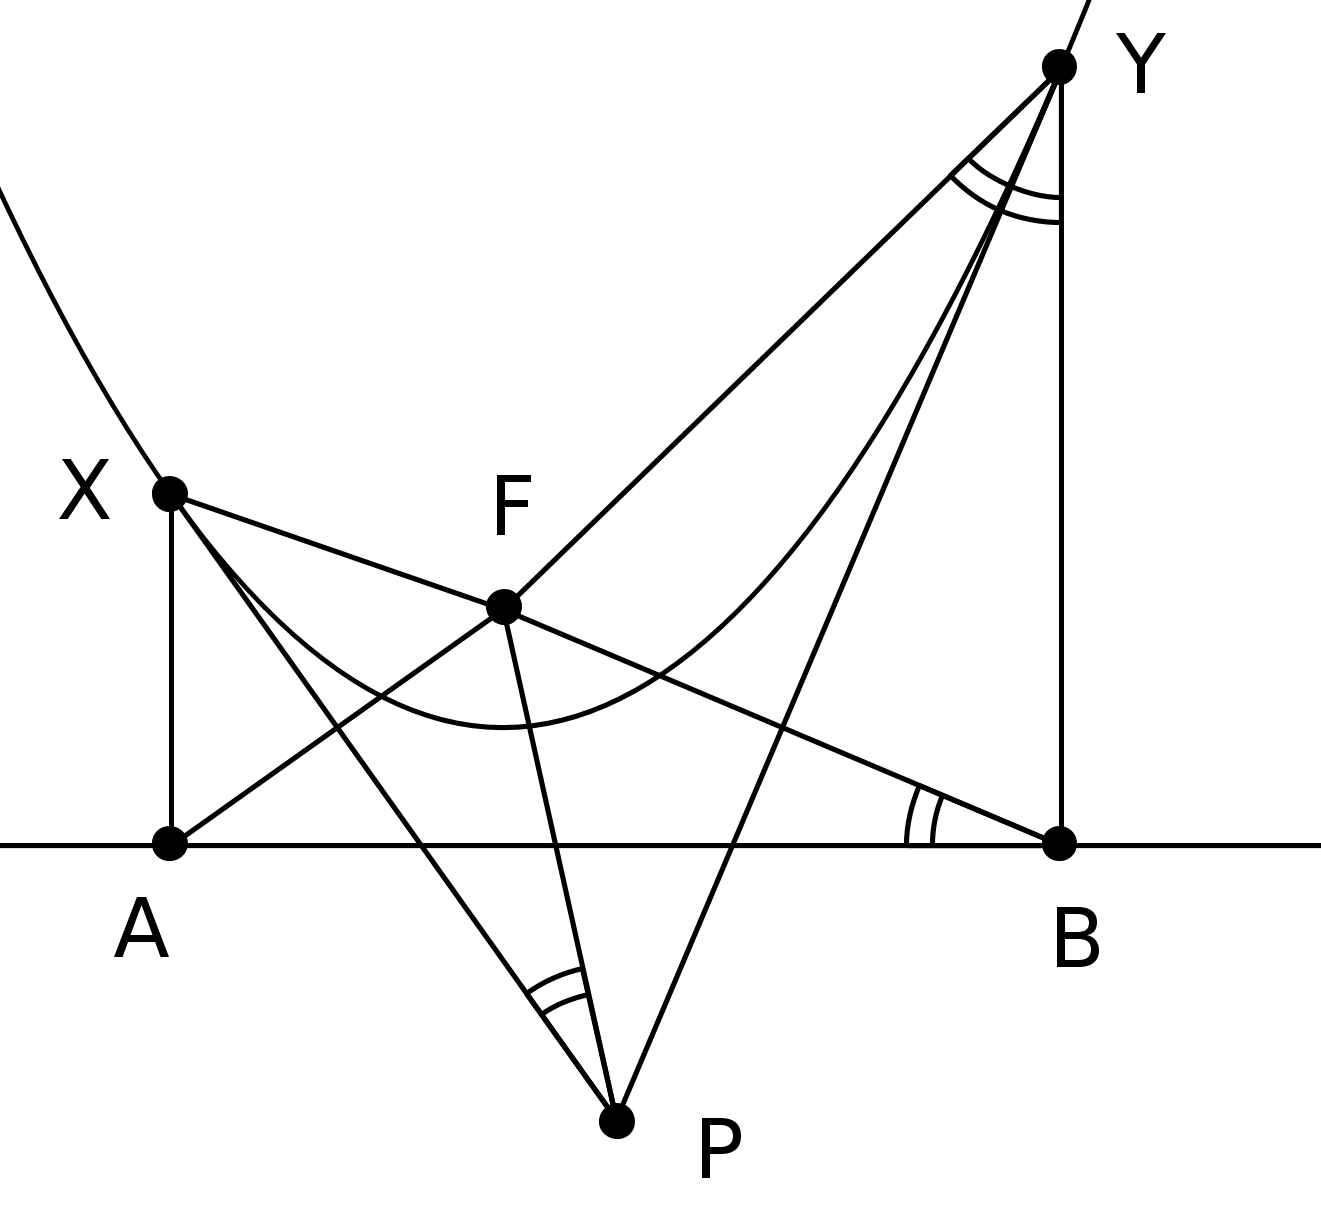
\includegraphics[width=0.5\linewidth]{pictures/2013-2014-bonus-6}
\end{center}

\item (Баев А.Ж.) Утверждение: $f^{2014}(x) = x$ имеет решение тогда и только тогда, когда $f(x) = x$ имеет решение. Легко доказывается от противного для произвольного уравнения $f^k(x) = x$ при $k>1$.

Пусть $f(x) \neq x$. Легко показать, что $f(x_v) > x_v$, где $x_v$ --- вершина параболы. Это значит, что множество значений $f(x)$ вложено в область возрастания $f(x)$. То есть $f(x) \geqslant f(x_{min}) > x_{min}$. Значит, минимальное значение $f^{k+1}(x)$ будет больше, чем минимальное значение $f^{k}(x)$.

\item (Баев А.Ж.) Композицией мы можем получить функции:
$$s(x) = \ctg (\arctg (x) ) = \frac{1}{x};$$
$$h(x) = \ctg (\arctg ( \cos ( \arctg(x) ) ) ) = \sqrt{x^2+1}.$$
Применив $k$ раз функцию $h(x)$, можно получить:
$$g_k(x) = h(h( ... h(x) ... )) = \sqrt{x^2 + k}.$$

Для всех $n \in \mathbb{N}, n > 1$ существует такое $k = n^2-1$, что $g_k(1) = n$. То есть, для любого натурального существует композиция такая, что  $R(1) = n$.

Рассмотрим 
$$g_2(s(x)) = \sqrt{\frac{1+2x^2}{x^2}}.$$
Если в качестве $x$ положить $n$ (из условия $m^2 - 2n^2 = 1$), то получим $g_2(s(n)) = \frac{m}{n}$.

\item Индукцией по $l$ доказывается, что
$$H_{2^l} = 1 + \frac{1}{2} + \frac{1}{3} + \hdots + \frac{1}{2^l} \leqslant l + 1.$$
Далее, с учетом того, что $p_i < 2^{100}$:
$$\left( \sum_{i=1}^{n} \frac{1}{p_i} \right)^k < k! \sum_{1 \leqslant i_1 \leqslant \hdots \leqslant i_n \leqslant n} \frac{1}{p_{i_1} p_{i_2} \hdots p_{i_k}} \leqslant $$
$$ \leqslant k! ( H_{2^{100k}} - 1) \leqslant (100 k) k!,$$
откуда
$$\sum_{i=1}^{n} \frac{1}{p_i} < \bigl( (100 k) \cdot k! \bigr) ^{\frac{1}{k}}.$$
Здесь $k$ --- любое натуральное. Положим $k = 4$.
\end{enumerate}



\end{document}